\documentclass[12pt]{article}

\usepackage[a4paper,margin=2cm]{geometry}

\usepackage{amsmath}
\usepackage{amssymb}
\usepackage{mathtools}

\usepackage{listings}

\usepackage{booktabs} % For tables
\usepackage[table,xcdraw]{xcolor} % For tables

\usepackage{enumerate}
\usepackage{enumitem}
\usepackage{tikz}
\usepackage{float}
\usepackage{nameref}
\usepackage{hyperref}
\usepackage{xcolor}

\definecolor{codegreen}{rgb}{0,0.6,0}
\definecolor{codegray}{rgb}{0.5,0.5,0.5}
\definecolor{codepurple}{rgb}{0.58,0,0.82}
\definecolor{backcolour}{rgb}{0.95,0.95,0.92}

\lstdefinestyle{mystyle}{
    backgroundcolor=\color{backcolour},
    commentstyle=\color{codegreen},
    keywordstyle=\color{magenta},
    numberstyle=\tiny\color{codegray},
    stringstyle=\color{codepurple},
    basicstyle=\ttfamily\footnotesize,
    breakatwhitespace=false,
    breaklines=true,
    captionpos=b,
    keepspaces=true,
    numbers=left,
    numbersep=5pt,
    showspaces=false,
    showstringspaces=false,
    showtabs=false,
    tabsize=2
}

\lstset{style=mystyle}

\DeclarePairedDelimiter\abs{\lvert}{\rvert}
\DeclarePairedDelimiter\Abs{\lVert}{\rVert}

\usepackage{fancyhdr}

\pagestyle{fancy}
\lhead{\today}
\chead{Exercise 03\\Algorithmic Foundations of Data Science}
\rhead{Fabian Grob\\Simon Michau\\Til Mohr}

\setlength{\headheight}{50pt}

\begin{document}

\section*{Exercise 1}
\begin{enumerate}[label= (\alph*)]
	\item	Using Theorem 3.6: With \(|\mathcal{H}| = 3^3 = 27\)
			\begin{align*}
				\Pr_{T ~ \mathcal{D}^m} &\left( \forall h \in \mathcal{H}: \abs{err_T(h) - err_D(h)} \leq \epsilon \right) > 1 - \delta \\
				\Pr_{T ~ \mathcal{D}^m} &\left( \forall h \in \mathcal{H}: \abs{err_T(h) - err_D(h)} \leq \epsilon \right) > 0.9 \\
				\Rightarrow &\delta = 0.1 \\\\
				m &\geq \frac{1}{2\epsilon^2} \log \left( \frac{2\abs{\mathcal{H}}}{\delta} \right) \\
				143 &\geq \frac{1}{2\epsilon^2} \log \left( \frac{2 \cdot 3^3}{0.1} \right) \\
				143 &\geq \frac{1}{2\epsilon^2} (\log(54) - \log(0.1)) \\
				143 &\geq \frac{1}{2\epsilon^2} (\log(54) - \log(0.1)) \\
				\epsilon^2 &\geq \frac{(\log(54) - \log(0.1))}{143 \dot 2} \\
				\abs{\epsilon} &\geq \sqrt{\frac{(\log(54) - \log(0.1))}{286}} \\
				\Rightarrow &\epsilon \geq \sqrt{\frac{(\log(54) - \log(0.1))}{286}} \\
				\Pr_{T ~ \mathcal{D}^m} &\left( \forall h \in \mathcal{H}: \abs{err_T(h) - err_D(h)} \leq \epsilon \right) > 0.9 \\
				\Pr_{T ~ \mathcal{D}^m} &\left( \forall h \in \mathcal{H}: \abs{0.03 - err_D(h)} \leq \sqrt{\frac{(\log(54) - \log(0.1))}{286}} \right) > 0.9 \\
				\Rightarrow &err_D(h) \leq 0.03 + \sqrt{\frac{(\log(54) - \log(0.1))}{286}} \simeq 0.208149 \simeq 0.21
			\end{align*}
	\item	Using Theorem 3.4:
			\begin{align*}
				\Pr_{T ~ \mathcal{D}^m} &\left( \forall h \in \mathcal{H}: \text{if $h$ is consistent with $T$, then } err_D(h) \leq \epsilon \right) 1 - \delta \\
				\Pr_{T ~ \mathcal{D}^m} &\left( \forall h \in \mathcal{H}: \text{if $h$ is consistent with $T$, then } err_D(h) \leq 0.01 \right) 0.9 \\
				\Rightarrow &\epsilon = 0.01, \delta = 0.1 \\\\
				m &\geq \frac{1}{\epsilon} \ln \left( \frac{\abs{\mathcal{H}}}{\delta} \right) \\
				m &\geq \frac{1}{0.01} \ln \left( \frac{3^3}{0.1} \right) \\
				m &\geq 100 (\ln(27) - \ln(0.1)) \simeq = 559.84 \\
				\Rightarrow &m \geq 560
			\end{align*}
\end{enumerate}


\section*{Exercise 2}

\section*{Exercise 3}

\section*{Exercise 4}
\begin{enumerate}[label= (\alph*)]
	\item See \refname{appendix} for code.
        \lstinputlisting{code/exercise_04_output.txt}
    \item No, the weights are always the same. This is because the loss matrix does not change throughout the algorithm, so the loss is always the same. 
        If all the events still happen in the sequence, only in a different order, this won't have an effect as the loss will still be included in the updated weight.
\end{enumerate}

\section*{Exercise 5}
\begin{enumerate}[label=(\alph*)]
	\item See \refname{appendix} for code.
        \lstinputlisting{code/exercise_05_output.txt}
    \item \(w_1^{(4)}\) and \(w_3^{(4)}\) are different because with \(\gamma = 0.5\) we put a certain weight on exploration.
        Therefore, even with the same reward, different actions can have different weights as \(\gamma\) is part of the weight updating calculation.
\end{enumerate}


\section*{Exercise 6}
\begin{enumerate}[label= (\alph*)]
    \item   \begin{enumerate}[label= (\roman*)]
                \item  \begin{figure}[H]
                            \centering
                            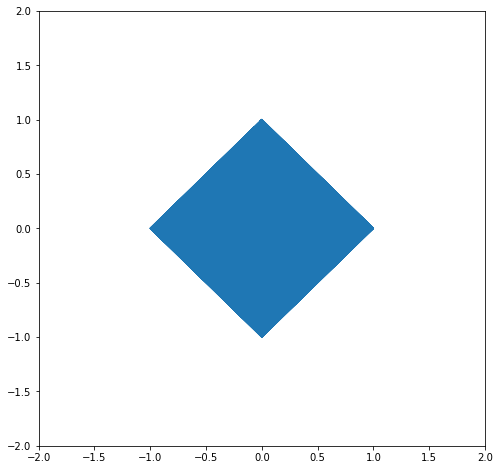
\includegraphics[width=3.5in]{unit_ball_plane.png}
                        \end{figure}
                \item The shape of \(B^3_1 \subset \mathcal{R}^3\) would look like a octahedron with the same edge length ($\sqrt{2}$).
            \end{enumerate}
    \item \(|diag(B^2_1)| = 2 \xRightarrow{\text{Pythagoras}} \text{edge length of }B^2_1 = \sqrt{2} \Rightarrow vol(B^2_1) = \sqrt{2}^2 = 2\) \\
        \(vol(B^3_1) = \frac{1}{3}\sqrt{2}a^3\) with $a$ being the edge length of the octahedron \(\Rightarrow vol(B^3_1) = \frac{1}{3}\sqrt{2}^4 = \frac{1}{3}4 = \frac{4}{3} \simeq  1.33\)\\
        A more general formula for the volume \(vol(B^l_1)\) is \(vol(B^l_1) = \frac{2^l}{l!}\) (cmp. this \href{https://doi.org/10.2307/30044198}{paper}).\\
        Using \(l = 1, 2\) yields the same results.
    \item 
        \begin{align*}
            &\lim_{l\rightarrow\inf}{\text{vol}(B^l_1) = \frac{2^l}{l!}}\\
            &\Rightarrow \lim_{l\rightarrow\inf}{\text{vol}(B^l_1)} = \frac{2}{1}\cdot \frac{2}{2}\cdot \frac{2}{3}\cdot \dotsb \cdot\frac{2}{l-1}\cdot \frac{2}{l}\\
            & \leq 2 \cdot \frac{2}{l}  = \frac{4}{l} \\
            &\Rightarrow \lim_{n\rightarrow\inf}{\frac{4}{l}} = 0
        \end{align*}

\end{enumerate}

    

\section*{Appendix}\label{appendix}
\subsection*{Code for Exercise 4}
\lstinputlisting[language=Python]{code/exercise_04.py}
\subsection*{Code for Exercise 5}
\lstinputlisting[language=Python]{code/exercise_05.py}
% \bibliographystyle{plainnat}
% \bibliography{\jobname}


\end{document}